\documentclass{report}
\usepackage{setspace}
\usepackage{graphicx}
\usepackage{amsthm}
\usepackage{amsmath}
\usepackage{hyperref}
\usepackage{tikz}
\usetikzlibrary{calc}
\numberwithin{equation}{chapter}

\begin{document}
\begin{center}
\begin{spacing}{1.5} { \textbf{ {\Large IMPLEMENTATION OF FINITE ELEMENT METHOD FOR PARABOLIC INTERFACE PROBLEM  \bigskip } } }
\end{spacing}
\bigskip \bigskip \bigskip \bigskip \bigskip A Project Report Submitted \\ in Partial Fulfilment of the Requirements for\\ \begin{spacing}{1.5} {\textbf{ \Large Summer Internship}}\end{spacing}
at \\ \begin{spacing}{1.5} {\textbf{ \Large Indian Institute Of Technology Guwahati \linebreak[5] }}
\end{spacing}
\bigskip\bigskip\bigskip\bigskip
by\\ Jinank Jain\\ (Roll No. UG201210017)\\ B.Tech, 2nd Year\\Computer Science and Engineering\\ Indian Institute Of Technology Jodhpur\\ \bigskip \bigskip

\includegraphics[scale=0.07]{iitg}\\ \bigskip to the\\ 
 \begin{spacing}{1.4} {\textbf{ \large DEPARTMENT OF MATHEMATICS \\ INDIAN INSTITUTE OF TECHNOLOGY GUWAHATI \\ GUWAHATI - 781039, INDIA\\ \bigskip}}\end{spacing}
 \textsl{July, 2014}
 
 % % % % % Certificate Page Begins Here
 \newpage
 {\textbf{ \Large CERTIFICATE\\ \bigskip}}
 \end{center}
 
 \begin{flushleft}
 This is to certify that the work contained in this project report entitled as \textbf{"Implementatiom of Finite Element Method for Parabolic Interface Problem"} \textbf{Jinank Jain (Roll No. UG201210017)} to Indian Institute of Technology towards partial requirement of \textbf{Summer Internship} which has been carried out by him under my supervision and that it has not been submitted elsewhere for the award of any degree.\\
 \end{flushleft}
 \bigskip \bigskip \bigskip \bigskip \bigskip
 
% \noindent \textbox{Guwahati - 781 039\hfill} \textbox{\hfill  (Dr. Rajen Kumar Sinha)}\\
% \noindent \textbox{July 2014\hfill} \textbox{\hfill  Project Supervisor} 
\noindent Guwahati - 781 039\hfill \hfill (Dr. Rajen Kumar Sinha)\\
\noindent July 2014\hfill \hfill Project Supervisor\\

% % % % Abstract Page Begins Here
\newpage
\begin{center}
 {\textbf{ \Large ABSTRACT\\ \bigskip}}
\end{center}
\begin{flushleft}
Finite Element Method is a numerical method for finding approximate solution to boundary value problems for differntial equation. It uses variational method to minimize an error function and produce a stable solution.
\end{flushleft}

% % % % Contents Page

\tableofcontents
\chapter{The Finite Element Method}
\section{Introduction}
\begin{spacing}{1.5}
From the ancient times, scientists and philosophers have been curious about different physical phenomenon occuring in the nature and have tried to understand and analyze the same. Almost every phenomenon today, whether simple or complex, can be described using the laws of physics with the help of mathematical modeling.\\ \\
\textbf{Definition 1.1.1} A mathematical model is a description of a system using mathematical concepts and language. The process of developing a mathematical model is termed \textsl{mathematical modeling}.\\ \\
Most of the practical problems of engineering involve very complex differential and/or integral equations posed on geometrically complicated domains. Solving and analyzing these models analaytically is too complex and will take much longer time. Howerever with the help of a computer ans some numerical methods it can be convenient to analyze these and it also proves to be very useful to analyze the effects of different paramaters on the system effectively. \\ \\
\textbf{Definition 1.1.2}  The study of algorithms that use numerical approximation for the problems of mathematical analysis is called a \textsl{numerical analysis}.\\ \\ 
There exists various numerical meyhods to solve the differential equations but the most powerful of these numerical methods is the \textbf{\textsl{finite element method} (or FEM)}. It is a technique for finding an approximate solution of boundary value and initial value problems characterized by partial differential equation. It produces a stable solution of the problem to minimize the error using the variational method.
\end{spacing}
\section{The Basic Idea}
\begin{spacing}{1.5}
The most distinctive feature of finite element method that seperates it from others is the division of a given domain into a set of simple subdomains, called finite elements. Any geometric shape that allows computation of the solution or its approximation, or provides necessary relations among the values of the solution at selected points, called nodes, of the subdomain, qualifies as finite element. Other features of the method include seeking continuous, often polynomial, approximations of the solution over each element in terms of nodal values, and assembly of elements equations by imposing the interelement continuity of the solution and balance of interelement forces.\\
There are three stages in the whole process where errors are generally introduced in most cases. The first is the partition of the domain into smaller subdomains and then assembling it back to generate the original domain which introduces some errors in the domain during the processs. Second stage is when element equations are derived. The dependent unknowns($u$) of the problem are approximated with the idea that any continous function can be represented by a linear combination of unknown functions $ \phi_{i} $ and undetermined coefficents $ c_{i} $ ( $ u \approx u_{h} = \Sigma {c_{i}\phi_{i}}$ ) . Algebraic relations among the undetermined coefficients  c$_{i}$ are obtained by satisfying the govering equations over each element in a weighted integral snese. The approximation functions $ \phi_{i}$ are often taken to be polynomails and are derived using the concepts from interpolation theory. Therefore they are termed as \textsl{interpolation functions. }So in the second stage , errors are introduced both in representing the solution $ u $ as well as in evaluating the integrals. And lastly errors are introduced in solving the assembled system of equations.
\end{spacing}
\section{Implementaion with Analysis}
\begin{spacing}{1.5}
To better understand how to implement the finite element method to a problem, we take an example from [11].\\ \\
\textbf{Example 1.3.1.} Approximation of the perimeter of a circle.\\
Consider the problem of determining the perimeter of a circle of radius R without using the formula ($P = 2\pi r$) for the perimater of a circle. Ancient mathematicians used to approximate value of the perimeter by straight line segments as $\pi$ was not known. Thus, the approximate value of the perimeter is obtained by adding the length pf the line segments used to represent it.\\
\begin{center}
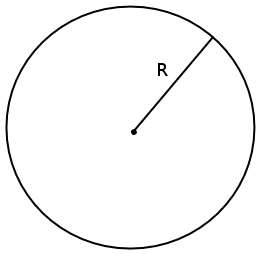
\includegraphics[scale=0.5]{circle}\\
Fig 1.1 A circle of radius R
\end{center}
With the help of this example we outline the basic ideas and steps involved in the finite element analysis of a problem.\\
\begin{description}
  \item[1. Finite Element Discretization:] First, the perimeter(domain of this problem) is divided into a collection of finite ($n$) number of subdoamins called line segments. This is called \textsl{discretization of the domain.} ome errors would be introduce here because we will need an infinite number of line elements to represent the exact perimeter. Each subdomain(i.e., line segment) is called an \textsl{element}. The collection of these elements is called \textsl{the finite element mesh}. The points at which elements are connected to each other are called \textsl{nodes}. In this case, we discretize the perimeter into a mesh of five line segments making $n$ = 5. The mesh is said to be uniform if all the elemnents are of same length; otherwise, it is called a \textsl{nonuniform} mesh.
  \begin{center}
  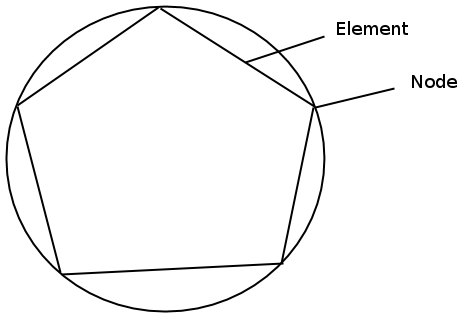
\includegraphics[scale=0.5]{circle1}\\
  Fig 1.2 Discretization of circle with n=5
  \end{center}
  \item[2. Element Equation:] An element(i.e., line segment, $\Omega_{e}$) is isolated and its required properties (length in this case) are computed by appropriate means. Let $h_{e}$ be the of the element $\Omega_{e}$ in the mesh. For a typical $\Omega_{e}$, $h_{e}$ is given by
  \begin{center}
  \begin{equation}
  	h_{e}= 2R\sin\frac{1}{2}\theta_{e}
  \end{equation}
  \end{center}
  where R is the radius of the circle and $\theta_{e} \textless \pi$ is the angle subtended by the line segement. The above equations are called \textsl{element equations.}
  \item[3. Assembly of elements equations and solutions:] The approximate value of the perimeter of the circle is obtained by putting together the element properties in a meaningful way and the process is known as the \textsl{assembly of the element equations.} In the present case it follows the property that the perimeter of the polygon $\Omega_{h}$(circle approximated by assembly of elements) is equal to the sum of the lengths of the individual elements:
  \begin{center}
    \begin{equation}
    	P_{n}= \sum_{e=1}^{n}h_{e}
    \end{equation}
    \end{center}
    Then $P_{n}$ represents an approximation to the actual perimeter, P. If the mesh is uniform, or $h_{e}$ is the same for each of the elements in the mesh, then $\theta_{e} = \frac{2\pi}{n}$, and we have
     \begin{center}
        \begin{equation}
        	P_{n} = n\left(2R\sin\frac{\pi}{n} \right)
        \end{equation}
     \end{center}
  \item[4. Convergence and error estimate:] Since we know the solution to this simple problem ($P = 2\pi R$), we can easily estimate the error in the approximation and show that the approximate solution $P_{n}$ converges to the exact value P as we increase the number of line segments used to approximate the perimeter(i.e., as $n \rightarrow \infty $). Consider a typical element $\Omega_{e}$. The error in the approximation is equal to the differnce between the length of the arc and that of the line segment
  \begin{center}
          \begin{equation}
          	E_{e} = \mid S_{e}-h_{e} \mid
          \end{equation}
       \end{center}
  where $S_{e} = R\theta_{e}$ is the arc length. Thus the error estimate for an element for an element in the mesh is given by
  \begin{center}
            \begin{equation}
            	E_{e} = R\left(\frac{2\pi}{n}-2\sin\frac{\pi}{n}\right)
            \end{equation}
  \end{center}
  The total error or the global error is given by multiplying $E_{e}$ by $n$:
  \begin{center}
              \begin{equation}
              	E = nE_{e} = 2R\left(\pi-n\sin\frac{\pi}{n}\right) = 2\pi R-P_{n} = P-P_{n}
              \end{equation}
    \end{center}
    We now show that E goes to zero as $n \rightarrow \infty$. Letting $x = \frac{1}{n}$, we have
    \begin{center}
         \begin{equation}
         P_{n} = 2Rn\sin\frac{\pi}{n} = 2R\frac{\sin\pi x}{x}         	
         \end{equation}
    \end{center}
    and
\begin{center}
         \begin{equation}
         \lim\limits_{n\rightarrow \infty}P_{n} =  \lim\limits_{n\rightarrow \infty}(2R\frac{\sin\pi x}{x}) = 2\pi R         	
         \end{equation}
\end{center}
\end{description}
\begin{center}

\end{center}
\end{spacing}
\section{Summary}
\begin{spacing}{1.5}
FEM is a numerical method to solve Boundary Value Problem(BVPs)(for e.g, structural and solid mechanics problem in engineering). The fundamental concept behind FEM is that any continous quantity such as temperature, pressure etc. can be approximated by a discrete model composed of a set of piecewise continous polynomial functions defined over a finite number of subdomains (elements). It has applications in areas like heat transfer, fluid mechnaics etc.\\ \\
\textbf{Advantages of the finite element method:}\\
\begin{itemize}
  \item Extensive application: applies to all physical problems in BVP or structural and solid mechanics.
  \item Application to composite materials: material properties in adjacent do not need to be same. 
  \item Applies to irregularly shaped boundaries as well: any boundary can be approximated using elements with straight sides or matched exactly using elements with curved boundaries.
  \item Scalable mesh: size of the elements can be vaired allowing the element grid or mesh to be expanded or refined as per the requirement.
  \item Mixed boundary conditions handling: boundary conditions such as discontinous surface loadings present no difficulties.
\end{itemize}
\textbf{Disadvantages and Limitations:}\\
\begin{itemize}
\item Gives solution only at nodal points.
\item Gives an approximate solution.
\end{itemize}
\end{spacing}

% % Chapter one complete
% % Chapter two starts here

\chapter{Finite Element Method: Parabolic Interface}
\section{Introduction}
\begin{spacing}{1.5}
The domain which we would consider for our study be rectangular domain $\Omega = (0,2)\times(0,1)$, having an interface at x = 1 such that $\Omega_{1} = (0,1)\times(0,1)$ and $\Omega_{2} = (1,2)\times(0,1)$. Consider the parabolic interface problem of the form:
 \begin{center}
    \begin{equation}
       u_{t}-\bigtriangledown.\left(\beta \bigtriangledown u \right) = f(u)
    \end{equation}
 \end{center}
 where $\beta$ is different at both side of equation. $\beta_{1} = 1$ for $x<1$ and $\beta_{2} = 0.5$ for $x>1$. The dirchelet boundary conditions are $u(x,0) = 0$, $u(x,1) = 0$, $u(0,y) = 0$ and $u(2,y) = 0$. Time varies from 0 to 0.1 s. The known soultion for u is given by:\\
  \begin{center}
     \begin{equation}
     	\begin{split}
     	u(x,y,t) = (exp(\sin t))(\sin\pi x . \sin\pi y) \qquad x<1 \\
     	u(x,y,t) = (exp(\sin t))(\sin 2\pi x . \sin\pi y) \qquad x>1
     	\end{split}
     \end{equation}
  \end{center}
	The value obtained for f using equation 2.1 and 2.2 is as follows:
 \begin{center}
     \begin{equation}
     	\begin{split}
     	f(x,y,t) = (exp(\sin t))(\sin\pi x . \sin\pi y)(\cos t + 2\pi^2) \qquad x<1 \\
     	f(x,y,t) = (-exp(\sin t))(\sin 2\pi x . \sin\pi y)(\cos t + 2.5\pi^2) \qquad x>1
     	\end{split}
     \end{equation}
  \end{center}
\end{spacing}
\section{Basic Data Structure Scheme}
\begin{spacing}{1.5}
The basic data structure scheme that we are going to follow during all implemntaion is as follows:
\begin{itemize}
\item For maintaing coordinates of nodal values we have made a file named c4n.mat (c4n stands for coordinates for nodes) which could be easily loaded using a simple octave command load filename.mat.
\item For maintaing node numbering of triangular elements which is always done in anticlockwise fashion is stored in file named n4e.mat (n4e stands for nodes for element).\\
\item For maintaining node numbering of dirchelet boundary value points we have made a filenamed n4sDb.mat(where n4sDb stands for nodes for dirchelet boundary)
\end{itemize}
\begin{center}
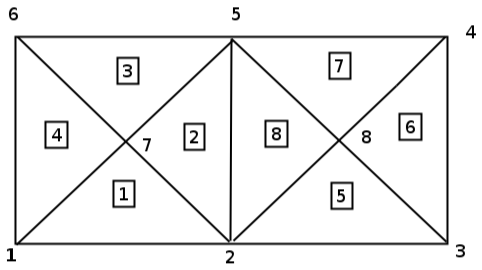
\includegraphics[scale=0.5]{mesh}\\
Fig 2.1 Sample mesh\\
Sample data stored in corresponding files for the given mesh in Fig 2.1\\
\begin{tabular}{l c r}
\hline c4n.mat & n4e.mat & n4sDb.mat \\
0  0 & 1 2 7 & 1 2\\
1  0 & 2 5 7 & 2 3\\
2  0 & 5 6 7 & 3 4\\
2  1 & 6 1 7 & 4 5\\
1  1 & 2 3 8 & 5 6\\
0  1 & 3 4 8 & 6 1\\
0.5  0.5 & 4 5 8\\
1.5  0.5 & 5 2 8\\
\end{tabular}
\end{center}
\end{spacing}
\section{Evaluation of Mass Matrix}
\begin{spacing}{1.5}
In order to evaluate mass matrix you need to follow this algorithm:\\
\noindent\rule{12cm}{0.4pt}\\
\textbf{Algorithm: Assembly of mass matrix}\\
\noindent\rule{12cm}{0.4pt}\\
\begin{itemize}
\item[1:] M = size of c4n
\item[2:] N = size of n4e
\item[3:] Allocate memory of size $M \times M$ to a matrix B and initialize all matrix entries to zero
\item[4:]\textbf{for} i = 1,2,3....,N \textbf{do}
\item[5:] Compute the $3\times3$ local element of mass matrix $B^I$ given by\\
\begin{center}
$G$ = $\begin{bmatrix}
       2 & 1 & 1 \\[0.3em]
       1 & 2 & 1 \\[0.3em]
       1 & 1 & 2
     \end{bmatrix}$\\
$B^{I}$ = $\frac{1}{24} \times G \times$ (Area of $i_{th}$ triangular element)
\end{center}
\item[6:] Add $B^{I}_{11}$ to $B_{ii}$
\item[7:] Add $B^{I}_{12}$ to $B_{ii+1}$
\item[8:] Add $B^{I}_{13}$ to $B_{ii+2}$
\item[9:] Add $B^{I}_{21}$ to $B_{i+1i}$
\item[10:] Add $B^{I}_{22}$ to $B_{i+1i+1}$
\item[11:] Add $B^{I}_{23}$ to $B_{i+1i+2}$
\item[12:] Add $B^{I}_{31}$ to $B_{i+2i}$
\item[13:] Add $B^{I}_{32}$ to $B_{i+2i+1}$
\item[14:] Add $B^{I}_{33}$ to $B_{i+2i+2}$
\item[15:] \textbf{end for}
\end{itemize}
\end{spacing}
\section{Evaluation of Stiffness Matrix}
\begin{spacing}{1.5}
In order to evaluate stiffness matrix you need to look into some details about triangulations.
For a trinagular element T let $(x_{1},y_{1})$, $(x_{2},y_{2})$ and $(x_{3},y_{3})$ be the vertices of the trinangle and $\eta_{1}$, $\eta_{2}$, and $\eta_{3}$ be the corresponding basis function in S, i.e.,
\begin{center}
$\eta_{j}(x_{k},y_{k}) = \delta_{jk},$ \qquad $j,k=1,2,3$
\end{center}
A moments reflection reveals\\
\begin{center}
$\eta_{j}(x,y) =$ det$
 \begin{pmatrix}
  1 & x  & y \\
  1 & x_{j+1} & y_{j+1} \\
  1  & x_{j+2} & y_{j+2} 
 \end{pmatrix}/$ det$\begin{pmatrix}
   1 & x_{j}  & y_{j} \\
   1 & x_{j+1} & y_{j+1} \\
   1  & x_{j+2} & y_{j+2} 
  \end{pmatrix}
$
\end{center}
whence
\begin{center}
$\nabla\eta_{j}(x,y) = \frac{1}{2|T|}
\begin{pmatrix}
y_{j+1}-y_{j+2}\\
x_{j+2}-x_{j+1}
\end{pmatrix}
$
\end{center}
Here, the indices are to be considered modulo 3, and $|T|$ is the area of T, i.e.,
\begin{center}
$2|T| = $ det$
\begin{pmatrix}
x_{2}-x_{1} & x_{3}-x_{1}\\
y_{2}-y_{1} & y_{3}-y_{1}
\end{pmatrix}
$
\end{center}
The resulting entry of stiffness matrix is
\begin{center}
$A_{jk} = \beta\int_{T} \nabla\eta_{j}(\nabla\eta_{k})^{T} dx$ = $\beta\frac{|T|}{4T^{2}}(y_{j+1}-y_{j+2}, x_{j+2}-x_{j+1})
\begin{pmatrix}
y_{k+1}-y_{k+2}\\
x_{k+2}-x_{k+1}
\end{pmatrix}
$
\end{center}
Here is the parameter $\beta$ is different on both sides of interface. This is written simultaneously for all indices as:
\begin{center}
$A = $ $\frac{|T|}{2}.GG^{T}$ with G:= $\begin{pmatrix}
1 & 1 & 1\\
x_{1} & x_{2} & x_{3} \\
y_{1} & y_{2} & y_{3}
\end{pmatrix}^{-1}$
$
\begin{pmatrix}
0 & 0\\
1 & 0\\
0 & 1
\end{pmatrix}
$
\end{center}
\noindent\rule{12cm}{0.4pt}\\
\textbf{Algorithm: Assembly of stifness matrix}\\
\noindent\rule{12cm}{0.4pt}\\
\begin{itemize}
\item[1:] M = size of c4n
\item[2:] N = size of n4e
\item[3:] Allocate memory of size $M \times M$ to a matrix A and initialize all matrix entries to zero
\item[4:] \textbf{for} i = 1,2,3...,N \textbf{do}
\item[5:] if T is on left hand side then take $\beta = 1$ else $\beta = 0.5$
\item[6:] Compute the 3$\times$3 local element of stiffness matrix $A^{I}$ as explained above with proper value of $\beta$.
\item[6:] Add $A^{I}_{11}$ to $A_{ii}$
\item[7:] Add $A^{I}_{12}$ to $A_{ii+1}$
\item[8:] Add $A^{I}_{13}$ to $A_{ii+2}$
\item[9:] Add $A^{I}_{21}$ to $A_{i+1i}$
\item[10:] Add $A^{I}_{22}$ to $A_{i+1i+1}$
\item[11:] Add $A^{I}_{23}$ to $A_{i+1i+2}$
\item[12:] Add $A^{I}_{31}$ to $A_{i+2i}$
\item[13:] Add $A^{I}_{32}$ to $A_{i+2i+1}$
\item[14:] Add $A^{I}_{33}$ to $A_{i+2i+2}$
\item[15:] \textbf{end for}
\end{itemize}
\end{spacing}
\section{Backward Euler Scheme}
\begin{spacing}{1.5}
First of all let us understand what is a basic backward euler scheme. Consider an ordinary differntial equation.
\begin{center}
$\frac{dy}{dt}$ = $f(t,y)$
\end{center}
with initial value $y(t_{o}) = y_{o}$. Here the function $f$ and the initial data $t_{o}$ and $y_{o}$ are known; the function $y$ depends on the real variable $t$ and is unknown. A numerical method produces a sequence $y_{0},y_{1},y_{2},....$ such that $y_{k}$ is approximates $y(t_{o}+kh)$, where h is called the step size. The backward Euler method computes the approximations using
\begin{center}
$y_{k+1}$ = $y_{k}$ + $hf(t_{k+1},y_{k+1})$
\end{center}
Now lets see how we implement this scheme for parabolic interface finite element method and see the assembly procedure.\\
The volume forces are used for assembling the right hand side. Using the value of $f$ in the center of gravity $(x_{s},y_{s})$ of $T$ the integral $\int_{T}f\eta_{j}dx$ is approximated using a proper curvature rule:
\begin{center}
$\int_{T}f\eta_{j}dx \approx$ = $\frac{1}{6}$det$
\begin{pmatrix}
x_{2}-x_{1} & x_{3}-x_{1}\\
y_{2}-y_{1} & y_{3}-y_{1}
\end{pmatrix}
$
$f(x_{s},y_{s})$
\end{center}
\noindent\rule{12cm}{0.4pt}\\
\textbf{Algorithm: Implementation of Backward Euler Scheme}\\
\noindent\rule{12cm}{0.4pt}\\
\begin{itemize}
\item[1:] M = size of c4n
\item[2:] N = size of n4e
\item[3:] Initialize b matrix of size M$\times$1, u matrix of size M$\times$1 and U matrix of size M$\times$(number of time steps+1)
\item[4:] \textbf{for} i = 1 to final time level \textbf{do}
\item[5:] \textbf{for} each triangular element calculate the volume force and add to b.
\item[6:] $b = b$ + $B$ * $U_{i-1}$ where B is mass matrix.
\item[7:] $b = b$ - ($dt*A$ + $B$)*u
\item[8:] $u$ = ($dt*A$ + $B$) * $b^{I}$
\item[9:] $U_{n}$ = $u$
\item[10:] \textbf{end for}
\end{itemize}
\end{spacing}
\section{Crank Nicklson Scheme}
\begin{spacing}{1.5}
First of all let us understand what is a basic crank nicklson scheme. Consider a partial differential equation:
\begin{center}
$\frac{\partial u}{\partial t}$ = $F(u,x,t,\frac{\partial u}{\partial x}, \frac{\partial^{2} u}{\partial x^{2}})$
\end{center}
then letting $u(i\triangle x, n\triangle t) = u_{i}^{n}$, the equation for 
Crank–Nicolson method is a combination of the forward Euler method at $n$ and the backward Euler method at$ n + 1$ (note, however, that the method itself is not simply the average of those two methods, as the equation has an implicit dependence on the solution):\\
\begin{center}
$\frac{u_{i}^{n + 1} - u_{i}^{n}}{\Delta t} = F_{i}^{n}\left(u,\, x,\, t,\, \frac{\partial u}{\partial x},\, \frac{\partial^2 u}{\partial x^2}\right) \qquad \mbox{(forward Euler)}
$\\
$\frac{u_{i}^{n + 1} - u_{i}^{n}}{\Delta t} = F_{i}^{n + 1}\left(u,\, x,\, t,\, \frac{\partial u}{\partial x},\, \frac{\partial^2 u}{\partial x^2}\right) \qquad \mbox{(backward Euler)}
$\\
$ \frac{u_{i}^{n + 1} - u_{i}^{n}}{\Delta t} = \frac{1}{2}\left[ F_{i}^{n + 1}\left(u,\, x,\, t,\, \frac{\partial u}{\partial x},\, \frac{\partial^2 u}{\partial x^2}\right) + F_{i}^{n}\left(u,\, x,\, t,\, \frac{\partial u}{\partial x},\, \frac{\partial^2 u}{\partial x^2}\right) \right].
$ 
\end{center}
\bigskip
Now lets see how we implement this scheme for parabolic interface finite element method and see the assembly procedure.\\
The volume forces are used for assembling the right hand side. Using the value of $f$ in the center of gravity $(x_{s},y_{s})$ of $T$ the integral $\int_{T}f\eta_{j}dx$ is approximated using a proper curvature rule:
\begin{center}
$\int_{T}f\eta_{j}dx \approx$ = $\frac{1}{6}$det$
\begin{pmatrix}
x_{2}-x_{1} & x_{3}-x_{1}\\
y_{2}-y_{1} & y_{3}-y_{1}
\end{pmatrix}
$
$f(x_{s},y_{s})$
\end{center}
\bigskip\bigskip\bigskip\bigskip\bigskip\bigskip\bigskip
\noindent\rule{12cm}{0.4pt}\\
\textbf{Algorithm: Implementation of Crank Nicklson Scheme}\\
\noindent\rule{12cm}{0.4pt}\\
\begin{itemize}
\item[1:] M = size of c4n
\item[2:] N = size of n4e
\item[3:] Initialize b matrix of size M$\times$1, u matrix of size M$\times$1 and U matrix of size M$\times$(number of time steps+1)
\item[4:] \textbf{for} i = 1 to final time level \textbf{do}
\item[5:] \textbf{for} each triangular element calculate the volume force and add to b.
\item[6:] $b = b$ + $(B-0.5*A*dt)$ * $U_{i-1}$ where B is mass matrix.
\item[7:] $b = b$ - $(B+0.5*A*dt)*u$
\item[8:] $u$ = $(B+0.5*A*dt)$ * $b^{I}$
\item[9:] $U_{n}$ = $u$
\item[10:] \textbf{end for}
\end{itemize}
\end{spacing}
\chapter{Conclusion}
\begin{spacing}{1.5}
We were able to demonstrate that the experimental order of conergences for various estimators such space, time, $L^{2}(\Omega)$ and $H^{1}$ were in harmony with the theortical results.\\
The finding of this experiment could be very much useful in study of various two heat conductors which have different heat conductivity or two fluids have different density and we could easily simulate these process with help of code developed during this project.\\
The things which could be further improved is that if we could deploy some advanced algorithms in refinement techniques so that they could be boost up and we could bring down the complexity of code. At last I would like to conclude on this fact that my project could contribute to some research aspects and could have some new findings.
\end{spacing}
\end{document}